\subsection{Protocols}\label{sec:protocols}

% (Preproject-copy)
This section will describe some of the protocols used by the \glspl{IDE} in \cref{sec:editors} and extensions in \cref{sec:extension-components}.

\subsubsection{JSON-RPC}

% (Preproject-copy)
\paragraph*{Description}
\emph{JSON-RPC} is a stateless \acrfull{RPC} protocol.
That means it allows one process to call \emph{procedures} (methods, subroutines, functions) in another process.
The format for serializing the calls' data is \gls{JSON}.
A key design goal is to be a simple protocol.~\cite{json-rpcworkinggroupJSONRPCSpecification2010}

% (Preproject-copy)
The protocol does not limit the \emph{transport mechanism} used, so \gls{JSON-RPC} could be sent inside the same process, across sockets, HTTP or any other form of message passing transport.~\cite{json-rpcworkinggroupJSONRPCSpecification2010}

% (Preproject-copy)
\paragraph*{Protocol}
The main definitions are data structures and error codes.
\Gls{JSON-RPC} defines a \texttt{Request} and \texttt{Response} object.~\cite{json-rpcworkinggroupJSONRPCSpecification2010}

% (Preproject-copy)
The Request must have an \texttt{id}, \texttt{method} name, \texttt{params} data structure and \texttt{jsonrpc} version field.
A Request without an \texttt{id} is a \texttt{Notification}, and will not get a Response back.~\cite{json-rpcworkinggroupJSONRPCSpecification2010}

% (Preproject-copy)
The Response must have an \texttt{id}, \texttt{result} or \texttt{error} data structure, and a \texttt{jsonrpc} version field.~\cite{json-rpcworkinggroupJSONRPCSpecification2010}


\subsubsection{Language Server Protocol (LSP)}\label{sec:lsp}

% (Preproject-copy)
\paragraph*{Goal} An \gls{IDE} often has to support many programming languages.
Most of the languages support some common features, such as autocomplete,  validation, definitions, references, renaming, selection etc..
The \gls{LSP} tries to separate language editor clients from language servers.
The clients are kept generic, while the language servers know the details for a programming language.~\cite{microsoftOverview}
This means a \gls{IDE} developer only needs to create \textit{one} editor, with generic \gls{LSP} support.
And a language developer only needs to create a language server.
If the language server adheres to the \gls{LSP} protocol, any \gls{LSP} client will automatically support it.
This is illustrated in \cref{fig:lsp-benefits}.

% (Preproject-copy)
\begin{figure}[htbp]  % order of priority: h here, t top, b bottom, p page
  \centering
  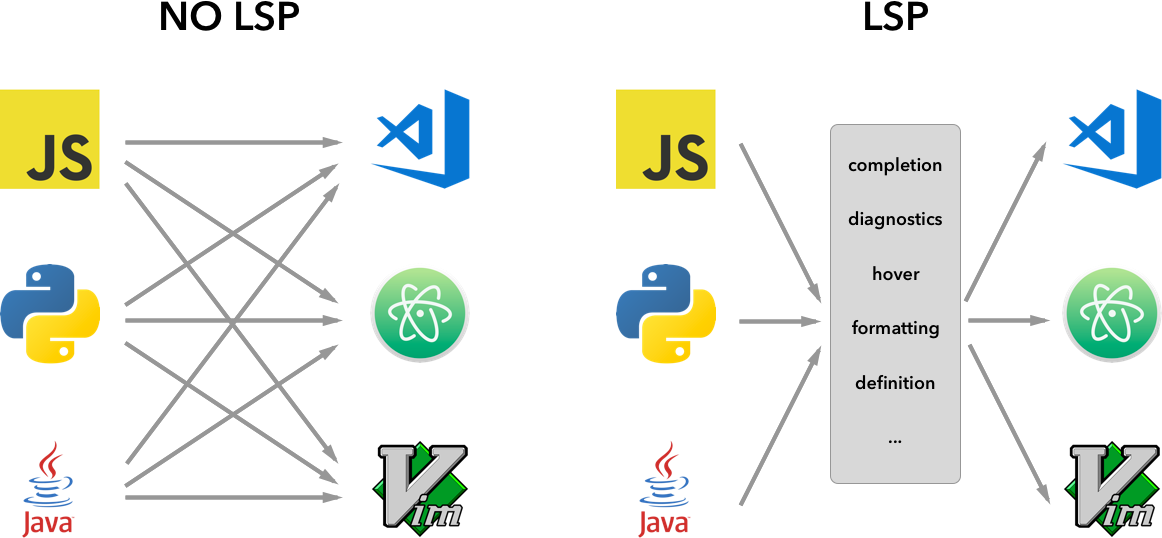
\includegraphics[width=\textwidth]{figures/lsp-languages-editors}
  \caption[LSP Benefits]{The benefits of using \gls{LSP}. There is no need for re-creating language support for every possible combination of editor and language.~\cite{microsoftLanguageServerExtension2020}}\label{fig:lsp-benefits}
\end{figure}


% (Preproject-copy)
\paragraph*{Details}
The protocol is based on a \emph{Base protocol}, which has a \texttt{key-value} \emph{header} and a \emph{content} with \gls{JSON-RPC} (see \cref{fig:lsp-protocol}).

% (Preproject-copy)
\begin{figure}[htbp]
  \centering
  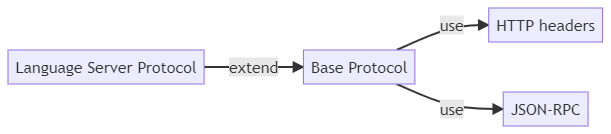
\includegraphics[width=\textwidth]{figures/lsp-protocol}
  \caption[The LSP Protocol]{The LSP protocol extends a Base protocol that uses HTTP headers and JSON-RPC content.}\label{fig:lsp-protocol}
\end{figure}

% (Preproject-copy)
\paragraph*{The Base protocol}
The header fields conform to the HTTP specification\footnote{RFC-7230 at \href{https://tools.ietf.org/html/rfc7230\#section-3.2}{https://tools.ietf.org/html/rfc7230\#section-3.2}.} with regards to structure and formatting.

% (Preproject-copy)
The Base protocol defines tree different message types that are sent in the \gls{JSON-RPC} content: \emph{Request}, \emph{Response} and \emph{Notification}.
There are also two key rules: every Request must be answered with a Response, and Notification does not need a Response.
The Base protocol provides a list of common error codes, extending the default error codes that \gls{JSON-RPC} provides.~\cite{microsoftLanguageServerProtocol2020}

% (Preproject-copy)
The Base protocol defines a rule for Request and Notification methods as well: a method starting with \texttt{\$/} is protocol implementation specific and therefore optional, meaning a client or server can skip implementing it if the method is not suitable\footnote{The example given is cancellation of asynchronous tasks in a server that is synchronous.}.~\cite{microsoftLanguageServerProtocol2020}

% (Preproject-copy)
Lastly, the Base protocol defines two Notifications: \texttt{\$/progress} and \texttt{\$/cancelRequest}.~\cite{microsoftLanguageServerProtocol2020}

% (Preproject-copy)
\paragraph*{The Language Server Protocol}
The actual \emph{Language Server Protocol} itself is a large collection of \gls{JSON-RPC} Request, Response and Notification messages sent over the Base protocol.
The protocol assumes that \textit{one} language server is used for \textit{one} language client.~\cite{microsoftLanguageServerProtocol2020}
This means a language server can not be shared between multiple clients.

% (Preproject-copy)
The protocol is tailored for textual languages and text documents.
It specifies a collection of data structures that should be used.
A central data structure is the \texttt{TextDocument}.
Inside a \texttt{TextDocument}, there can be \texttt{Location}s in the text, and \texttt{Range}s of text between two \texttt{Location}s.
Changing a \texttt{TextDocument} is done by constructing a \texttt{TextDocumentEdit}, which holds a list of text replacements in \texttt{TextEdit}s, and a pointer to a \texttt{TextDocument} version using a \texttt{VersionedTextDocumentIdentifier}.
A \texttt{TextEdit} has \texttt{Range} to edit and a string with the new text.~\cite{microsoftLanguageServerProtocol2020}
An illustration of the data structures are shown in \cref{fig:lsp-data-structures}.
Note that this is only a small subset of the data structures defined in \gls{LSP}\footnote{Most of the supported features are described at \href{https://code.visualstudio.com/api/language-extensions/language-server-extension-guide\#additional-language-server-features}{https://code.visualstudio.com/api/language-extensions/language-server-extension-guide\#additional-language-server-features}.}.

% (Preproject-copy)
\begin{figure}[htbp]
  \centering
  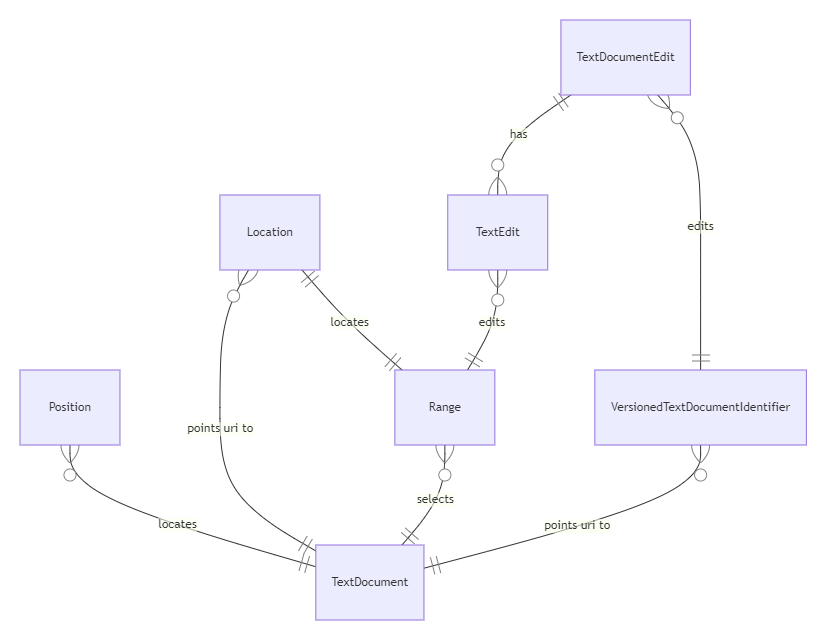
\includegraphics[width=\textwidth]{figures/lsp-textdocument-data}
  \caption[LSP Central Data Structures]{Central data structures in \gls{LSP}.}\label{fig:lsp-data-structures}
\end{figure}


\subsubsection{Graphical Language Server Platform (GLSP)}\label{sec:glsp}

% (Preproject-copy)
\paragraph*{Goal}
The \emph{Eclipse \gls{GLSP}} tries to create an analogous protocol to \gls{LSP}, but for graphical diagram editors.
It wants to be a solution for reusable \emph{graphical} language servers as well as generic clients.~\cite{jonashelmingGraphicalLanguageServer2019}
An illustration of \gls{GLSP} is shown in \cref{fig:glsp-overview}.

% (Preproject-copy)
\begin{figure}[htbp]  
  \centering
  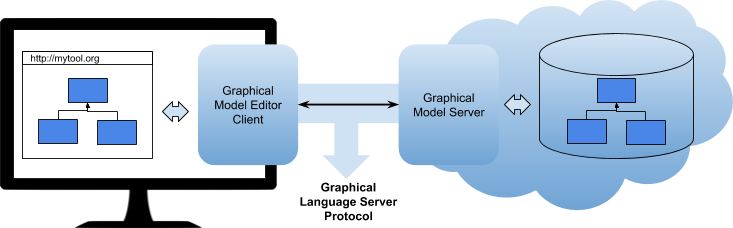
\includegraphics[width=\textwidth]{figures/glsp-overview.png}
  \caption[GLSP Overview]{An overview of the \gls{GLSP}.~\cite{eclipsefoundationGLSP2020}}\label{fig:glsp-overview}
\end{figure}

% (Preproject-copy)
\paragraph*{Details}
Being a platform, it aims a bit wider than the \gls{LSP} protocol by providing several implementations.
The platform has client and server implementations that speak the \gls{GLSP} protocol, and integrations into some \glspl{IDE}.
The client deals with rendering and user feedback, for example during drag-and-drop.
The server handles the diagram logics, validation and layouting.~\cite{jonashelmingGraphicalLanguageServer2019}

% (Preproject-copy)
The client uses technologies like Sprotty (\cref{sec:sprotty}), Typescript and \acrshort{svg}.
The server uses java, and has an existing integration with \gls{emf}.~\cite{eclipsefoundationGLSP2020}

% (Preproject-copy)
\paragraph*{The protocol}
The protocol is based around client-server communication over \gls{JSON-RPC}.
As with \gls{LSP}, one server is only responsible for one client.
The messages sent are inspired by the protocol used by Sprotty, but extended with user editing capabilities.~\cite{philiplangerEclipseglspGlspPROTOCOL2020}

% (Preproject-copy)
A core concept of the protocol is \emph{Action}, which is sent in a \emph{ActionMessage}.
All communication happends by sending Actions.
Actions are identified by a \texttt{kind}, and can be mapped to a concrete Action implementation by this kind.~\cite{philiplangerEclipseglspGlspPROTOCOL2020}
There are four main types of action: \emph{RequestAction}, \emph{ResponseAction}, \emph{RejectAction} and \emph{Operation}.
A RequestAction must be answered by a ResponseAction or rejected by a RejectAction.
Operations are requests from the client to modify the model.
Modifications are always done on the server.~~\cite{philiplangerEclipseglspGlspPROTOCOL2020}

% (Preproject-copy)
The protocol defines a large collection of Actions and Operations, to cover all needs of a graphical editor\footnote{A list of \gls{GLSP} features are listed at: \href{https://github.com/eclipse-glsp/glsp\#features}{https://github.com/eclipse-glsp/glsp\#features}.}.

